\section{Organization and Management}
\label{sec:fdsp-tpcelec-management}

In this Section we first discuss the organization of the \dword{ce}
consortium that at the moment consists entirely of US institutions, 
fifteen university groups plus groups from four DOE national 
laboratories. Table~\ref{tab:SPCE:institutions} provides a list 
of the participating institutions and the contact people at each institution. 
Later we discuss the assumptions that have been made in developing
the construction plan for the detector components that will be
provided by the \dword{ce} consortium, including the responsibilities
of the different institutions that are part of the consortium. Finally
we present a schedule for the construction, integration, and installation
of the detector, including an estimate of the resources required.

\begin{dunetable}
[Participating intitutes]
{p{0.15\textwidth}p{0.45\textwidth}}
{tab:SPCE:institutions}
{Institutes participating in the \dword{ce} consortium.}
ID & Institution \\ \toprowrule
 1 & Brookhaven National Laboratory \\ \colhline
 2 & Boston University \\ \colhline
 3 & University of Chicago \\ \colhline
 4 & University of Cincinnati \\ \colhline
 5 & Colorado State University  \\ \colhline
 6 & Columbia University \\ \colhline
 7 & University of California, Davis \\ \colhline
 8 & Fermi National Accelerator Laboratory \\ \colhline
 9 & University of Florida \\ \colhline
10 & University of Hawaii \\ \colhline
11 & Iowa State University \\ \colhline
12 & University of California, Irvine \\ \colhline
13 & Lawrence Berkeley National Laboratory \\ \colhline
14 & Louisiana State University \\ \colhline
15 & Michigan State University \\ \colhline
16 & University of Pennsylvania \\ \colhline
17 & University of Pittsburgh \\ \colhline
18 & SLAC National Accelerator Laboratory \\ \colhline
19 & Stony Brook University \\
\end{dunetable}
%% \begin{dunetable}
%% [Participating intitutes]
%% {p{0.15\textwidth}p{0.75\textwidth}}
%% {tab:SPCE:institutions}
%% {Institutes participating in the \dword{ce} consortium.}
%% ID & Institution \\ \toprowrule
%% ID & Institution (Contact person with E-mail) \\ \toprowrule
%%  1 & Brookhaven National Laboratory (\href{mailto:mworcester@bnl.gov}{Matt Worcester}) \\ \colhline
%%  2 & Boston University (\href{mailto:kearns@bu.edu}{Ed Kearns}) \\ \colhline
%%  3 & University of Chicago (\href{mailto:dwschmitz@uchicago.edu}{David Schmitz}) \\ \colhline
%%  4 & University of Cincinnati (\href{mailto:alex.sousa@uc.edu}{Alexander Sousa}) \\ \colhline
%%  5 & Colorado State University (\href{mailto:mrmooney@colostate.edu}{Michael Mooney}) \\ \colhline
%%  6 & Columbia University (\href{mailto:georgia@nevis.columbia.edu}{Georgia Karagiorgi}) \\ \colhline
%%  7 & University of California, Davis (\href{mailto:mulhearn@physics.ucdavis.edu}{Michael Mulhearn}) \\ \colhline
%%  8 & Fermi National Accelerator Laboratory (\href{mailto:dcc@fnal.gov}{David Christian}) \\ \colhline
%%  9 & University of Florida (\href{mailto:ikfuric@ufl.edu}{Ivan Furic}) \\ \colhline
%% 10 & University of Hawaii (\href{mailto:varner@uhawaii.edu}{Gary Varner}) \\ \colhline
%% 11 & Iowa State University (\href{mailto:krennrich@iastate.edu}{Frank Krennrich}) \\ \colhline
%% 12 & University of California, Irvine (\href{mailto:bianjm@uci.edu}{Jianming Bian}) \\ \colhline
%% 13 & Lawrence Berkeley National Laboratory (\href{mailto:cjslin@lbl.gov}{ChengJu Lin}) \\ \colhline
%% 14 & Louisiana State University (\href{mailto:mtzanov@lsu.edu}{Martin Tzanov}) \\ \colhline
%% 15 & Michigan State University (\href{mailto:bromberg@pa.msu.edu}{Carl Bromberg}) \\ \colhline
%% 16 & University of Pennsylvania (\href{mailto:cmauger@penn.edu}{Christopher Mauger}) \\ \colhline
%% 17 & University of Pittsburgh (\href{mailto:vipres@pitt.edu}{Vittorio Paolone}) \\ \colhline
%% 18 & SLAC National Accelerator Laboratory (\href{mailto:convery@slac.stanford.edu}{Mark Convery}) \\ \colhline
%% 19 & Stony Brook University (\href{mailto:alpinist@nngroup.physics.sunysb.edu}{Chang Kee Jung}) \\
%%\end{dunetable}

%%%%%%%%%%%%%%%%%%%%%%%%%%%%%%%%%%%
\subsection{Consortium Organization}
\label{sec:fdsp-tpcelec-management-consort}

The present consortium organization
structure includes a leader and a technical lead (both currently
from \dword{fermilab}), with personnel from \dword{bnl} helping with system design. A working group structure has been recently 
provided with subgroups responsible for the detector 
components inside the cryostat (\dwords{asic}, \dwords{femb}, and
cold cables), outside the cryostat (mostly the \dwords{wiec} with 
their boards), and all equipment
used for testing the detector components. When appropriate, subgroups
responsible for integration at the \dword{itf} and
\dword{surf} will be formed (for now, the technical lead oversees 
these activities). In addition,
another subgroup will be in charge of software and physics
preparation activities, including calibrations and simulations.
Mechanical design activities span detector components both inside
and outside the cryostat, requiring strong contacts between 
Technical Coordination and other consortia (mainly the \dword{apa}
consortium). The lead engineer (from \dword{bnl}) on mechanical aspects of the cold
electronics (mechanical interfaces with the \dwords{apa}, cabling, including 
cable trays, cryostat penetrations) works directly with
the Technical Coordination team. The \dword{ce} consortium will also have 
contact people for the overall \dword{lbnf}/\dword{dune} management for
\dword{esh} and for \dword{qa}/\dword{qc}. For the moment, the technical lead oversees these activities although oversight
will be transferred in part to each subgroup leader for testing
activities. The leadership positions in the consortium 
%% The current contact people for the various leadership positions in the consortium
are listed in Table~\ref{tab:SPCE:leadership}.

%% \begin{dunetable}
%% [Leadership positions in the Consortium]
%% {p{0.45\textwidth}p{0.45\textwidth}}
%% {tab:SPCE:leadership}
%% {Current leadership positions in the \dword{ce} consortium.}\
%% Position & Responsible person (with E-mail) \\ \toprowrule
%% Leader & \href{mailto:dcc@fnal.gov}{David Christian} (Fermilab) \\ \colhline
%% Technical Lead & \href{mailto:mverzocc@fnal.gov}{Marco Verzocchi} (Fermilab) \\ \colhline
%% System Aspects & \href{mailto:chc@bnl.gov}{Hucheng Chen} (Brookhaven) \\ \colhline
%% Cold Components & \href{mailto:mverzocc@fnal.gov}{Marco Verzocchi} (Fermilab) \\ \colhline
%% Warm Components & \href{mailto:mworcester@bnl.gov}{Matt Worcester} (Brookhaven) \\ \colhline
%% Test Setups & \href{mailto:ikfuric@ufl.edu}{Ivan Furic} (Florida) \\ \colhline
%% Mechanical Design & \href{mailto:mzhao@bnl.gov}{Manhong Zhao} (Brookhaven) \\ \colhline
%% Reliability Task Force & \href{mailto:varner@uhawaii.edu}{Gary Varner} (Hawaii) \\ \colhline
%% TDR Editor & \href{mailto:mrmooney@colostate.edu}{Michael Mooney} (Colorado State) \\ \colhline
%% \dword{esh} contact & \href{mailto:mverzocc@fnal.gov}{Marco Verzocchi} (Fermilab) \\ \colhline
%% \dword{qa}/\dword{qc} contact & \href{mailto:ikfuric@ufl.edu}{Ivan Furic} (Florida) and
%%                       \href{mailto:mverzocc@fnal.gov}{Marco Verzocchi} (Fermilab) \\ \colhline
%% \end{dunetable}
\begin{dunetable}
[Leadership positions in the Consortium]
{p{0.35\textwidth}}
{tab:SPCE:leadership}
{Current leadership positions in the \dword{ce} consortium.}\
Position \\ \toprowrule
Leader \\ \colhline 
Technical Lead \\ \colhline 
System Aspects \\ \colhline 
Cold Components \\ \colhline 
Warm Components \\ \colhline 
Test Setups \\ \colhline 
Mechanical Design \\ \colhline 
Reliability Task Force \\ \colhline 
TDR Editor \\ \colhline 
\dword{esh} contact \\ \colhline 
\dword{qa}/\dword{qc} contact \\ \colhline 
\end{dunetable}

In addition to the working groups, task forces for specific issues 
will be formed as necessary. A first example is the task force
charged with studying reliability issues in the \dword{ce} 
components and preparing recommendations for the choice of 
\dwords{asic}, the design of printed circuit boards, and testing; this
was discussed in Section~\ref{sec:fdsp-tpcelec-qa-reliability}. 
Later this task force will help in developing the \dword{qc} 
program for the \dword{ce} detector components, in collaboration
with the testing group leadership, starting from the \dword{pdsp} 
experience. Later, a second task force, with possible
personnel overlap with the first task force and possibly including experts
from outside the \dword{dune} Collaboration, will be tasked with establishing the
criteria for the \dword{asic} selection. This task force will
be also asked to propose a recommendation that will then go to
the \dword{dune} Executive Board for the final approval, as discussed
in Section~\ref{sec:fdsp-tpcelec-design-femb-selection}.

%%%%%%%%%%%%%%%%%%%%%%%%%%%%%%%%%%%
\subsection{Planning Assumptions}
\label{sec:fdsp-tpcelec-management-planning}

In Section~\ref{sec:fdsp-tpcelec-management-cost}, we describe
the current schedule for the construction, integration, and installation
of the \dword{ce} detector components for the first \dword{sp} \dword{tpc} \dword{fd}. This schedule, and the costs associated
with detector construction, are based on experience with constructing and commissioning the \dword{pdsp}
detector and on assumptions for the remaining R\&D program
and the production planning discussed here. 
Section~\ref{sec:fdsp-tpcelec-production-spares} details
the number of spare parts that we plan to fabricate to
account for known yield issues during detector construction
and to address possible problems. Table~\ref{tab:SPCE:components}
gives a summary of all fabricated components, and where
appropriate tested, required for the first \dword{sp}
\dword{tpc} \dword{fd}. To develop a schedule for detector construction, 
we must then consider the current state of development of 
the \dwords{asic}. \dwords{femb}, and all other components to 
estimate the time required for final development of these
two components.

A second detector may be built using the \dword{sp} technology, 
and in that vase the construction of the \dword{ce} components 
for the second detector would immediately follow construction of 
the first detector. The total number of components for the second 
detector will be less than for the first detector, assuming that, 
for components inside the cryostat, the spare parts from the first 
detector can be used for the second detector. Similarly, for the 
components on the top of the cryostat, the
pool of spares from the first detector should be sufficient to cover
the second detector.

\begin{dunetable}[Number of CE components required 
	for a \dword{spmod} TPC] %the Single Phase \dword{tpc} \dword{fd}] (and dword for CE too long)
{p{0.5\textwidth}p{0.5\textwidth}}
{tab:SPCE:components}
{Number of \dword{ce} components required for a \dword{spmod} TPC %the single phase \dword{tpc} \dword{fd} 
(accounting for spares and yield).}
Component & Number required \\ \toprowrule
\dword{fe} ASIC & 30,000 chips (at least 43 wafers) \\ \colhline
\dword{coldadc} and \dword{coldata} & 30,000 and 7,500 chips (at least 33 wafers) \\ \colhline
\dword{cryo} & 7,500 chips (at least 35 wafers) \\ \colhline
\dword{femb} & 3,200 \\ \colhline
Cold signal cables & 1,650 and 1,575 (bottom and top \dword{apa}) \\ \colhline
Cold power cables & 1,650 and 1,575 (bottom and top \dword{apa}) \\ \colhline
Cold bias voltage cables & 660 and 630 (bottom and top \dword{apa}) \\ \colhline
Cryostat penetrations & 80 \\ \colhline
\dword{ce} flanges & 160 \\ \colhline
\dword{wiec} & 155 \\ \colhline
\dword{wib} & 775 \\ \colhline
\dword{ptc} & 155 \\ \colhline
Warm power cables & 165 (3 different lengths) \\ \colhline
Warm bias voltage cables & 1,320 (3 different lengths) \\ \colhline
Wiener PL506 power box & 30 \\ \colhline
Wiener MPOD crate & 30 \\ \colhline
Wiener MPOD modules with 8 HV channels & 180 \\ \colhline
Power supplies and cables for heaters and fans & 30 \\ \colhline
\end{dunetable}

The critical path for the construction of the first \dword{sp}
\dword{tpc} \dword{fd} is driven by the availability of \dwords{femb},
which in turn depends on completing the design of the
\dwords{asic}. Thus, construction
of the \dword{apa}s could start as early as Spring 2020, while the
decision on the \dwords{asic} to be used on the \dwords{femb}
may come as late as Fall 2020. The schedule for this decision
depends on the \dword{ce} consortium, which is
planning a second design iteration on all \dwords{asic}
followed by system tests of various flavors of \dwords{femb}.
The first version of all \dwords{asic} will undergo
standalone tests in Spring 2019 and then will go through the 
sequence of system tests (with the 40\% \dword{apa} prototype at \dword{bnl},
the seventh \dword{pdsp} \dword{apa} in the cold box at CERN
and the \dword{tpc} in the \dword{iceberg} cryostat at \dword{fermilab})
during Summer 2019. At the same time, lifetime tests will be performed 
on all \dwords{asic}. Designs of the \dwords{asic} and \dwords{femb}, including results
from the system test stands and from lifetime tests will be reviewed
in early Fall 2019. This will trigger any further design
changes on the \dwords{asic} and then the second round of prototyping
and testing. This gets us to the Fall 2020 date for the final
\dword{asic} decision. Consequently, the initial
tests of the \dword{dune} prototype \dword{apa}s must be performed
with preliminary versions of \dwords{femb}, which will still be using
the first generation of \dwords{asic} although the final 
mechanical and electrical connections to the \dwords{apa} will be available and used.

After the Fall 2020 review, an additional six months may be 
required for a final iteration of the \dword{femb} design
and a final round of system tests before beginning fabrication
of the \dwords{asic} and \dwords{femb}. Engineering runs
for the \dwords{asic} and \dwords{femb} should then take place in the
second half of 2021, with most production starting in
Spring 2022. Depending on which solution is chosen for the
\dwords{asic}, production and testing of all chips required
for constructing the first \dword{sp} \dword{tpc} \dword{fd}
would be in hand by Spring or Summer 2023. The first batch of
production \dword{femb} would then be available for installation on
the \dword{apa}s in Winter 2023, and production would be
completed in Fall 2024, roughly six month after completing
fabrication of the \dwords{apa} for the first detector.
This schedule assumes that during construction of the 
\dword{apa}s, integration tests will be performed using preliminary
versions of the \dwords{femb} that must then be replaced
with final versions later. Integrating the \dwords{femb}
with the \dword{apa}s would be completed a couple of months after
the final set of \dwords{femb} is delivered to \dword{itf}.

If a second \dword{sp} \dword{tpc} \dword{fd} is built, the critical
path will transition from the \dwords{femb}
to the \dword{apa}s, assuming that construction
of both \dword{apa}s and \dwords{femb} will continue 
without interruption after construction of the first detector. 
This is because constructing one \dword{apa} requires 
more time than constructing the corresponding \dwords{femb}. Therefore,
toward the end of the constructing this possible second detector,
we expect that all required \dwords{femb} will be at the
\dword{itf} waiting for the delivery of the \dwords{apa} before
integration can take place.

All other detector components that are the responsibility of the
\dword{ce} consortium can be produced relatively quickly
in less than two years. The procurement, assembly, and
testing of these components can be scheduled so that
we have sufficient time in the schedule to address possible 
problems during production. Changes in all these
components, unlike those used in the \dword{pdsp} detector,
are less important than those affecting the \dwords{asic}
and \dwords{femb}. We are assuming that final
designs for the rest of the detector components will be 
available in the second half of 2020 and that the corresponding 
Production Readiness Reviews will occur, at the latest, six months 
before the \dword{asic} choice.
The first components 
required for installing the detector are the cryostat 
penetrations, which must be installed before the 
detector support structure inside the cryostat is completed.
In this way, the cryostat can be completely sealed, other than
the manholes used to feed clear air into the cryostat
and for the \dword{tco} used to exhaust the air flow
and as an entry point for the detector components. The rest of the
\dword{ce} components, which are installed on top of the 
cryostat (\dwords{wiec} with all their boards, supplies, cables
and fibers), should be installed before installing
the corresponding rows of \dword{apa}s and properly connecting 
the \dword{apa}s to power, control, and read-out. 
The \dword{apa}s should be tested as soon as they are installed. 

%%%%%%%%%%%%%%%%%%%%%%%%%%%%%%%%%%%
\subsection{Institutional Responsibilities}
\label{sec:fdsp-tpcelec-management-resp}

Design and prototyping for the \dword{sp} \dword{dune} detector have been 
concentrated so far at the DOE national laboratories, mostly because the 
focus was on designing the new generation of \dwords{asic}. The design 
of the \dword{fe} \dword{asic} was done at \dword{bnl}, \dword{cryo} 
chip at \dword{slac}, and the new \dword{coldadc} was a joint effort of 
\dword{bnl}, \dword{fermilab}, and \dword{lbnl}. The \dword{coldata} 
\dword{asic} was designed at \dword{fermilab}, with some components 
provided by engineers from the Electrical Engineering Department
at Southern Methodist University (not a consortium member).
The \dword{cts} was designed at Michigan State University.
Most of the design and construction work for the \dword{pdsp} detector 
was done at \dword{bnl}, with other institutions contributing to 
testing, installation, and commissioning. Given the extent of the project, 
particularly testing, additional institutions have begun to contribute
to all activities for constructing the \dword{sp} detector, which began 
in the middle of 2018. Almost all the engineering of detector components, 
except for the boards to be installed on the \dwords{wiec} and most boards 
and set ups for testing, will remain a responsibility
of the DOE national laboratories. Testing of 
\dwords{asic}, \dwords{femb}, cables, power and bias voltage supplies,
\dwords{wiec} with their boards will be done at various
universities that are members of a consortium. All institutions
are expected to contribute to the integration activities at
the \dword{itf} and to the installation at \dword{surf}, which is very
demanding in terms of personnel. A detailed list of the 
institutions contributing to the development, production, and
testing of the various detector components is given below.
\metainfo{The assignment of responsibilities within the consortium
is still under discussion, with an expected first draft available
in Spring 2019. At that time additional information will be
added here.}

%%%%%%%%%%%%%%%%%%%%%%%%%%%%%%%%%%%
\subsection{High-Level Cost and Schedule}
\label{sec:fdsp-tpcelec-management-cost}

\metainfo{Some dates in the following depend on the actual LBNF
schedule for the cryostat, that is still under revision. Therefore,
we are not specifying these dates at this point and indicate them
with 20XX. We expect to put updated information in this Section
after the January 2019 DUNE Collaboration Meeting, possibly in
time for the submission of the second draft of the TDR to the LBNC.}

In Section~\ref{sec:fdsp-tpcelec-management-planning}, we  
discussed how the project will evolve from the current design
and prototyping phase to production for the \dwords{asic}
and \dwords{femb} by Spring 2022. During the same  
period, the engineering of all other detector components will
be completed and prototypes fabricated. The procurement
and qualification of cold cables, cryostat penetrations, \dwords{wiec},
and power and bias voltage supplies can then begin in Spring 2021.
Integrating \dwords{femb} on the \dword{apa}s would then
take place over 18 months beginning in early 2023. At
this moment, the installing and testing of \dword{apa}s in 
the cryostat and corresponding activities of the \dword{ce} consortium, including installing all 
detector components on top of the cryostat, are scheduled to
take YY months starting in Spring 20XX. Table~\ref{tab:SPCE:timeline} shows a preliminary list of 
milestones, including the current plan to complete  
the design, R\&D, and engineering phase, and then later  
the production setup and production, integration,
and installation activities.

\begin{dunetable}
[\dword{ce} consortium milestones]
{p{0.15\textwidth}p{0.75\textwidth}}
{tab:SPCE:timeline}
{Milestones of the \dword{ce} consortium.}
\textbf{Date} & \textbf{Milestone} \\ \toprowrule
Feb 2019 & Complete the submission of the first generation of \dwords{asic} \\ \colhline
Aug 2019 & Complete the standalone testing of the first generation of \dwords{asic} \\ \colhline
Nov 2019 & Complete system and lifetime tests on the first generation of \dwords{asic} and \dwords{femb} \\ \colhline
Jan 2020 & Submission of second generation of \dwords{asic} \\ \colhline
Jul 2020 & Complete the standalone testing of the first generation of \dwords{asic} \\ \colhline
Nov 2020 & Complete system and lifetime tests on the second generation of \dwords{asic} and \dwords{femb} \\ \colhline
Nov 2020 & Decision on the \dword{asic}(s) to be used for construction \\ \colhline
May 2021 & Complete characterization of final prototypes of \dwords{asic} and \dwords{femb} including system tests \\  \colhline
Jul 2021 & Complete Engineering Design Reviews and launch pre-production of detector components \\ \colhline 
Oct 2021 & Complete installation of \dwords{femb} on \dword{pdsp} \dwords{apa} \\ \colhline
Dec 2021 & Complete testing of pre-production of all \dwords{asic} \\ \colhline
Mar 2022 & Complete testing of pre-production \dwords{femb} \\ \colhline
Mar 2022 & Complete testing of prototypes and Production Readiness Reviews \\ \colhline
May 2022 & Set-up of \dword{ce} test equipment at the \dword{itf} complete \\ \colhline
Feb 2023 & Begin installation of \dwords{femb} on \dwords{apa} at the \dword{itf} \\ \colhline
Mar 2023 & Procurement and testing of all detector components except \dwords{asic} and \dwords{femb} complete \\ \colhline
Aug 2023 & Construction and testing of \dwords{asic} complete \\ \colhline
Jan 2024 & Construction and testing of \dwords{femb} complete \\ \colhline
Sep 2024 & Integration of \dword{ce} components with \dwords{apa} complete \\ \colhline
Mar 20XX & Begin installation and testing of \dword{ce} components at \surf \\ \colhline
Jan 20YY & Installation of \dword{ce} components complete \\ \colhline
Aug 20YY & Complete testing and monitoring of detector prior to cryostat cool-down and filling \\ \colhline
Jun 20ZZ & Begin detector commissioning with cosmics \\ \colhline
Sep 20ZZ & Commissioning of detector complete \\ \colhline
\end{dunetable}

A detailed estimate of the \dword{ce} project costs was done in Summer/Fall 2018, using as a starting point
the actual expenses for constructing the \dword{pdsp}
detector. Thus, a large fraction of construction
cost estimates are on very solid ground because most of the detector components 
need only minor changes from the \dword{pdsp} design. While the
set of \dwords{asic} used for constructing the \dwords{femb}
will be completely new, the cost of the \dwords{femb} can
be estimated reliably using the \dword{pdsp} estimates,
once the cost of the \dword{fpga} is subtracted from the total
(fabrication cost of the printed circuit board,
cost of the discrete components, and the assembly cost
will not be significantly different). The same holds true
for the \dwords{wib} even if its design is altered significantly
from \dword{pdsp}.
The cost drivers for the \dwords{wib} are fabricating
printed circuit boards, the components (including
optical transmitters and receivers that are not going to change),
the \dword{fpga}, and the assembly. The \dwords{asic} set will
be completely new, but the fabrication costs are well
known because the prototyping and fabrication of
\dwords{asic} are performed using frame contracts, either
through MOSIS in the US or through IMEC in Europe, which
have fixed costs for production, while costs in the engineering
phase depend only on the size of the chip. One item that
changes significantly for \dword{dune} is the cryostat penetration,
where the spool piece changes from a T-shape to a cross-shape.
Even before completing the engineering of the spool piece
the cost increase can be estimated reliably by
scaling the cost by a factor of 33\% which reflects the increase
in the amount of tubing and the welding necessary to build
the spool piece. 

Overall the biggest uncertainty in cost is
in the prototyping phase, where we assume we need  a second
iteration only of the \dwords{asic} and \dwords{femb} prototypes
before moving to pre-production of 
components. The other main uncertainty in the cost of the
project relates to preparing all the testing
equipment required both during the prototyping phase and
during the construction and qualification of the detector
components. These cost uncertainties are not sizable 
relative to the overall cost of all the \dword{ce}
detector components.

An estimate of the construction costs for the first \dword{sp}
\dword{tpc} \dword{fd}, including all costs for prototyping and
pre-production starting from January 2020, is in Table~\ref{tab:SPCE:costs}.
\metainfo{This is for the moment a place holder. There has to
be an agreement with the Neutrino Cost Group on how to present
these costs, and whether only CORE costs should be presented in
this table. The table format below is a proposal from the
\dword{ce} consortium that needs to be discussed with
the DUNE management and with the Neutrino Cost Group. The starting date also
needs to be discussed.}

\begin{dunetable}
[Construction costs for the \dword{ce} detector components]
{lrrr}
{tab:SPCE:costs}
{Construction costs for the \dword{ce} detector components during the various phases of the project.}
Component & Prototyping & Pre-production & Production \\ \toprowrule
\dwords{asic} & & & \\ \colhline
\dwords{femb} & & & \\ \colhline
Cold cables & & & \\ \colhline
Cryostat penetrations & & & \\ \colhline
\dwords{wiec}, \dwords{wib}, \dwords{ptc} & & & \\ \colhline
Power and bias voltage supplies & & & \\ \colhline
Test stands & & & \\ \colhline
Integration & & & \\ \colhline
Installation & & & \\ \colhline
\end{dunetable} 

The estimates for labor are also based on 
experience from \dword{pdsp} construction. We assume that by testing multiple \dwords{asic}
at once and automating the testing process itself,
both for \dwords{asic} and \dwords{femb}, will reduce personnel needs for these tasks. 
Integration activities at the \dword{itf} and \dword{surf}
will be more complex than for \dword{pdsp} and
will require more personnel. A complete estimate of the
personnel needs for the integration and installation tasks
requires a better definition of the responsibilities of
the various consortia (\dword{apa}, \dword{hv}, \dword{pds},
\dword{daq}, and \dword{cisc}) and of the underground
installation team for all activities taking place
at \dword{surf}. Personnel needs for the project are listed in
Table~\ref{tab:SPCE:personnel} for the prototyping,
pre-production, and construction phases. Personnel
needs are expressed in terms of \dword{fte}
for each of five job categories: graduate students,
post-docs, scientists, engineers, and technicians. Only the
integral number of \dword{fte}-years in each job category is given
in Table~\ref{tab:SPCE:personnel}. Distributions of the number of \dwords{fte} as
a function of time, without differentiation between the
phases of the project are given in Figure~\ref{fig:SPCE:ftedist}.
\metainfo{The format of the table needs to be agreed upon with
the DUNE management and the Neutrino Cost Group. This table
will not be available before Spring 2019, as it depends on
the update of the DOE project schedule, that will happen on
that scale. The figure mentioned in the text will be made
available at the same time. The current one is a temporary 
place holder.}

\begin{dunefigure}
[Personnel needs for the \dword{ce} construction as a function of time]
{fig:SPCE:ftedist}
{Personnel needs for the construction of the \dword{ce} detector components 
as a function of time for different job categories.}
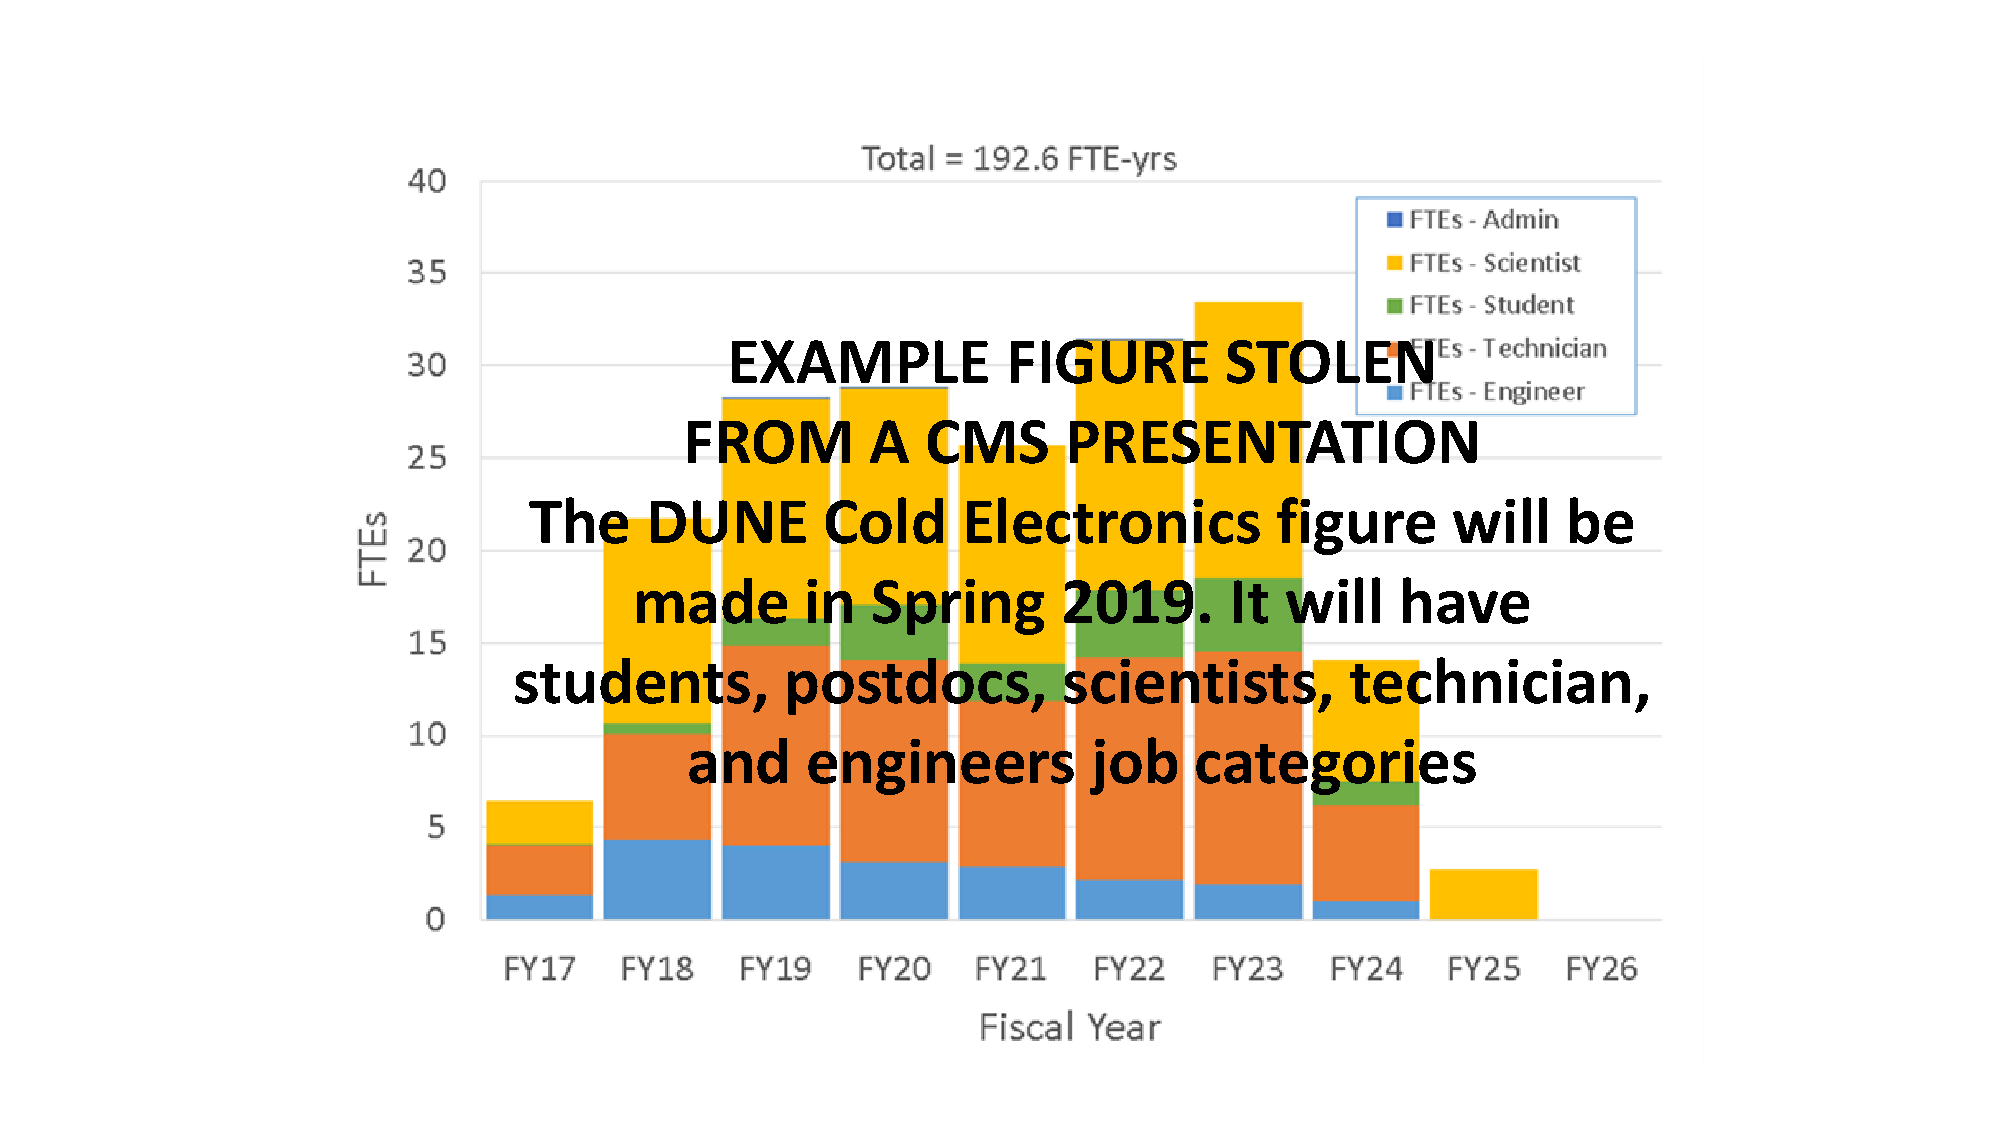
\includegraphics[width=0.8\linewidth]{sp-tpcelec-personnel-vs-time.pdf}
\end{dunefigure}

\begin{dunetable}
[Personnel needs for the \dword{ce} consortium]
{lrrrrr}
{tab:SPCE:personnel}
	{Personnel needs (in \dword{fte}--years) for the construction of the \dword{ce} detector 
components, their integration and installation for different job categories and 
in different project phases.}
Component & Students & Postdocs & Scientists & Engineers & Technicians \\
\rowcolor{dunetablecolor}
\multicolumn{6}{c}{Prototyping phase} \\ \toprowrule
\dwords{asic} & & & & & \\ \colhline
\dwords{femb} & & & & &  \\ \colhline
Cold cables & & & & & \\ \colhline
Cryostat penetrations & & & & & \\ \colhline
\dwords{wiec}, \dwords{wib}, \dwords{ptc} & & & & & \\ \colhline
Power and bias voltage supplies & & & & & \\ \colhline
Test stands & & & & & \\ 
\rowcolor{dunetablecolor}
\multicolumn{6}{c}{Pre-production phase} \\ \toprowrule
\dwords{asic} & & & & & \\ \colhline
\dwords{femb} & & & & &  \\ \colhline
Cold cables & & & & & \\ \colhline
Cryostat penetrations & & & & & \\ \colhline
\dwords{wiec}, \dwords{wib}, \dwords{ptc} & & & & & \\ \colhline
Power and bias voltage supplies & & & & & \\ \colhline
Test stands & & & & & \\ \colhline
Integration & & & & & \\
\rowcolor{dunetablecolor}
\multicolumn{6}{c}{Construction phase} \\ \toprowrule
\dwords{asic} & & & & & \\ \colhline
\dwords{femb} & & & & &  \\ \colhline
Cold cables & & & & & \\ \colhline
Cryostat penetrations & & & & & \\ \colhline
\dwords{wiec}, \dwords{wib}, \dwords{ptc} & & & & & \\ \colhline
Power and bias voltage supplies & & & & & \\ \colhline
Test stands & & & & & \\ \colhline
Integration & & & & & \\ \colhline
Installation & & & & & \\ \colhline
\end{dunetable}
